% Options for packages loaded elsewhere
% Options for packages loaded elsewhere
\PassOptionsToPackage{unicode}{hyperref}
\PassOptionsToPackage{hyphens}{url}
\PassOptionsToPackage{dvipsnames,svgnames,x11names}{xcolor}
%
\documentclass[
  letterpaper,
  DIV=11,
  numbers=noendperiod]{scrartcl}
\usepackage{xcolor}
\usepackage{amsmath,amssymb}
\setcounter{secnumdepth}{5}
\usepackage{iftex}
\ifPDFTeX
  \usepackage[T1]{fontenc}
  \usepackage[utf8]{inputenc}
  \usepackage{textcomp} % provide euro and other symbols
\else % if luatex or xetex
  \usepackage{unicode-math} % this also loads fontspec
  \defaultfontfeatures{Scale=MatchLowercase}
  \defaultfontfeatures[\rmfamily]{Ligatures=TeX,Scale=1}
\fi
\usepackage{lmodern}
\ifPDFTeX\else
  % xetex/luatex font selection
\fi
% Use upquote if available, for straight quotes in verbatim environments
\IfFileExists{upquote.sty}{\usepackage{upquote}}{}
\IfFileExists{microtype.sty}{% use microtype if available
  \usepackage[]{microtype}
  \UseMicrotypeSet[protrusion]{basicmath} % disable protrusion for tt fonts
}{}
\makeatletter
\@ifundefined{KOMAClassName}{% if non-KOMA class
  \IfFileExists{parskip.sty}{%
    \usepackage{parskip}
  }{% else
    \setlength{\parindent}{0pt}
    \setlength{\parskip}{6pt plus 2pt minus 1pt}}
}{% if KOMA class
  \KOMAoptions{parskip=half}}
\makeatother
% Make \paragraph and \subparagraph free-standing
\makeatletter
\ifx\paragraph\undefined\else
  \let\oldparagraph\paragraph
  \renewcommand{\paragraph}{
    \@ifstar
      \xxxParagraphStar
      \xxxParagraphNoStar
  }
  \newcommand{\xxxParagraphStar}[1]{\oldparagraph*{#1}\mbox{}}
  \newcommand{\xxxParagraphNoStar}[1]{\oldparagraph{#1}\mbox{}}
\fi
\ifx\subparagraph\undefined\else
  \let\oldsubparagraph\subparagraph
  \renewcommand{\subparagraph}{
    \@ifstar
      \xxxSubParagraphStar
      \xxxSubParagraphNoStar
  }
  \newcommand{\xxxSubParagraphStar}[1]{\oldsubparagraph*{#1}\mbox{}}
  \newcommand{\xxxSubParagraphNoStar}[1]{\oldsubparagraph{#1}\mbox{}}
\fi
\makeatother

\usepackage{color}
\usepackage{fancyvrb}
\newcommand{\VerbBar}{|}
\newcommand{\VERB}{\Verb[commandchars=\\\{\}]}
\DefineVerbatimEnvironment{Highlighting}{Verbatim}{commandchars=\\\{\}}
% Add ',fontsize=\small' for more characters per line
\usepackage{framed}
\definecolor{shadecolor}{RGB}{241,243,245}
\newenvironment{Shaded}{\begin{snugshade}}{\end{snugshade}}
\newcommand{\AlertTok}[1]{\textcolor[rgb]{0.68,0.00,0.00}{#1}}
\newcommand{\AnnotationTok}[1]{\textcolor[rgb]{0.37,0.37,0.37}{#1}}
\newcommand{\AttributeTok}[1]{\textcolor[rgb]{0.40,0.45,0.13}{#1}}
\newcommand{\BaseNTok}[1]{\textcolor[rgb]{0.68,0.00,0.00}{#1}}
\newcommand{\BuiltInTok}[1]{\textcolor[rgb]{0.00,0.23,0.31}{#1}}
\newcommand{\CharTok}[1]{\textcolor[rgb]{0.13,0.47,0.30}{#1}}
\newcommand{\CommentTok}[1]{\textcolor[rgb]{0.37,0.37,0.37}{#1}}
\newcommand{\CommentVarTok}[1]{\textcolor[rgb]{0.37,0.37,0.37}{\textit{#1}}}
\newcommand{\ConstantTok}[1]{\textcolor[rgb]{0.56,0.35,0.01}{#1}}
\newcommand{\ControlFlowTok}[1]{\textcolor[rgb]{0.00,0.23,0.31}{\textbf{#1}}}
\newcommand{\DataTypeTok}[1]{\textcolor[rgb]{0.68,0.00,0.00}{#1}}
\newcommand{\DecValTok}[1]{\textcolor[rgb]{0.68,0.00,0.00}{#1}}
\newcommand{\DocumentationTok}[1]{\textcolor[rgb]{0.37,0.37,0.37}{\textit{#1}}}
\newcommand{\ErrorTok}[1]{\textcolor[rgb]{0.68,0.00,0.00}{#1}}
\newcommand{\ExtensionTok}[1]{\textcolor[rgb]{0.00,0.23,0.31}{#1}}
\newcommand{\FloatTok}[1]{\textcolor[rgb]{0.68,0.00,0.00}{#1}}
\newcommand{\FunctionTok}[1]{\textcolor[rgb]{0.28,0.35,0.67}{#1}}
\newcommand{\ImportTok}[1]{\textcolor[rgb]{0.00,0.46,0.62}{#1}}
\newcommand{\InformationTok}[1]{\textcolor[rgb]{0.37,0.37,0.37}{#1}}
\newcommand{\KeywordTok}[1]{\textcolor[rgb]{0.00,0.23,0.31}{\textbf{#1}}}
\newcommand{\NormalTok}[1]{\textcolor[rgb]{0.00,0.23,0.31}{#1}}
\newcommand{\OperatorTok}[1]{\textcolor[rgb]{0.37,0.37,0.37}{#1}}
\newcommand{\OtherTok}[1]{\textcolor[rgb]{0.00,0.23,0.31}{#1}}
\newcommand{\PreprocessorTok}[1]{\textcolor[rgb]{0.68,0.00,0.00}{#1}}
\newcommand{\RegionMarkerTok}[1]{\textcolor[rgb]{0.00,0.23,0.31}{#1}}
\newcommand{\SpecialCharTok}[1]{\textcolor[rgb]{0.37,0.37,0.37}{#1}}
\newcommand{\SpecialStringTok}[1]{\textcolor[rgb]{0.13,0.47,0.30}{#1}}
\newcommand{\StringTok}[1]{\textcolor[rgb]{0.13,0.47,0.30}{#1}}
\newcommand{\VariableTok}[1]{\textcolor[rgb]{0.07,0.07,0.07}{#1}}
\newcommand{\VerbatimStringTok}[1]{\textcolor[rgb]{0.13,0.47,0.30}{#1}}
\newcommand{\WarningTok}[1]{\textcolor[rgb]{0.37,0.37,0.37}{\textit{#1}}}

\usepackage{longtable,booktabs,array}
\newcounter{none} % for unnumbered tables
\usepackage{calc} % for calculating minipage widths
% Correct order of tables after \paragraph or \subparagraph
\usepackage{etoolbox}
\makeatletter
\patchcmd\longtable{\par}{\if@noskipsec\mbox{}\fi\par}{}{}
\makeatother
% Allow footnotes in longtable head/foot
\IfFileExists{footnotehyper.sty}{\usepackage{footnotehyper}}{\usepackage{footnote}}
\makesavenoteenv{longtable}
\usepackage{graphicx}
\makeatletter
\newsavebox\pandoc@box
\newcommand*\pandocbounded[1]{% scales image to fit in text height/width
  \sbox\pandoc@box{#1}%
  \Gscale@div\@tempa{\textheight}{\dimexpr\ht\pandoc@box+\dp\pandoc@box\relax}%
  \Gscale@div\@tempb{\linewidth}{\wd\pandoc@box}%
  \ifdim\@tempb\p@<\@tempa\p@\let\@tempa\@tempb\fi% select the smaller of both
  \ifdim\@tempa\p@<\p@\scalebox{\@tempa}{\usebox\pandoc@box}%
  \else\usebox{\pandoc@box}%
  \fi%
}
% Set default figure placement to htbp
\def\fps@figure{htbp}
\makeatother





\setlength{\emergencystretch}{3em} % prevent overfull lines

\providecommand{\tightlist}{%
  \setlength{\itemsep}{0pt}\setlength{\parskip}{0pt}}



 


\KOMAoption{captions}{tableheading}
\makeatletter
\@ifpackageloaded{caption}{}{\usepackage{caption}}
\AtBeginDocument{%
\ifdefined\contentsname
  \renewcommand*\contentsname{Table of contents}
\else
  \newcommand\contentsname{Table of contents}
\fi
\ifdefined\listfigurename
  \renewcommand*\listfigurename{List of Figures}
\else
  \newcommand\listfigurename{List of Figures}
\fi
\ifdefined\listtablename
  \renewcommand*\listtablename{List of Tables}
\else
  \newcommand\listtablename{List of Tables}
\fi
\ifdefined\figurename
  \renewcommand*\figurename{Figure}
\else
  \newcommand\figurename{Figure}
\fi
\ifdefined\tablename
  \renewcommand*\tablename{Table}
\else
  \newcommand\tablename{Table}
\fi
}
\@ifpackageloaded{float}{}{\usepackage{float}}
\floatstyle{ruled}
\@ifundefined{c@chapter}{\newfloat{codelisting}{h}{lop}}{\newfloat{codelisting}{h}{lop}[chapter]}
\floatname{codelisting}{Listing}
\newcommand*\listoflistings{\listof{codelisting}{List of Listings}}
\makeatother
\makeatletter
\makeatother
\makeatletter
\@ifpackageloaded{caption}{}{\usepackage{caption}}
\@ifpackageloaded{subcaption}{}{\usepackage{subcaption}}
\makeatother
\usepackage{bookmark}
\IfFileExists{xurl.sty}{\usepackage{xurl}}{} % add URL line breaks if available
\urlstyle{same}
\hypersetup{
  pdftitle={Texas Flood Exposure Analysis},
  pdfauthor={Maya Arnott},
  colorlinks=true,
  linkcolor={blue},
  filecolor={Maroon},
  citecolor={Blue},
  urlcolor={Blue},
  pdfcreator={LaTeX via pandoc}}


\title{Texas Flood Exposure Analysis}
\usepackage{etoolbox}
\makeatletter
\providecommand{\subtitle}[1]{% add subtitle to \maketitle
  \apptocmd{\@title}{\par {\large #1 \par}}{}{}
}
\makeatother
\subtitle{A spatial and statistical assessment of flood risk across
Texas counties, 2019--2024}
\author{Maya Arnott}
\date{2026-03-23}
\begin{document}
\maketitle

\renewcommand*\contentsname{Table of contents}
{
\setcounter{tocdepth}{3}
\tableofcontents
}

\section{Overview}\label{overview}

This project quantifies flood exposure and risk across Texas's 254
counties over the period 2019--2024, combining live government data
sources, GIS spatial analysis, hydrological frequency modeling, and
regression to produce a reproducible county-level flood risk index.

The analysis is split across two Python modules:

\begin{itemize}
\tightlist
\item
  \textbf{\texttt{texas\_flood\_analysis.py}} --- data pipeline, spatial
  joins, and visualizations
\item
  \textbf{\texttt{risk\_modeling.py}} --- flood frequency distributions,
  regression modeling, and the final risk index
\end{itemize}

All data is either fetched programmatically from public APIs at run time
or from

\begin{center}\rule{0.5\linewidth}{0.5pt}\end{center}

\section{Data Sources}\label{data-sources}

{\def\LTcaptype{none} % do not increment counter
\begin{longtable}[]{@{}
  >{\raggedright\arraybackslash}p{(\linewidth - 4\tabcolsep) * \real{0.3333}}
  >{\raggedright\arraybackslash}p{(\linewidth - 4\tabcolsep) * \real{0.3333}}
  >{\raggedright\arraybackslash}p{(\linewidth - 4\tabcolsep) * \real{0.3333}}@{}}
\toprule\noalign{}
\begin{minipage}[b]{\linewidth}\raggedright
Source
\end{minipage} & \begin{minipage}[b]{\linewidth}\raggedright
Data
\end{minipage} & \begin{minipage}[b]{\linewidth}\raggedright
Access
\end{minipage} \\
\midrule\noalign{}
\endhead
\bottomrule\noalign{}
\endlastfoot
FEMA OpenFEMA API & NFIP flood insurance claims by county, 2019--2024 &
Public REST API \\
USGS NWIS & Annual peak streamflow, full historical record & Public REST
API \\
Census TIGER & County boundaries (254 Texas counties) &
\texttt{pygris} \\
Robbie M Parks and Victoria D Lynch & PRISM County-Level Precipitation
Data & Github Download upon Request \\
Multi-Resolution Land Characteristics (MRLC) Consortium & Impervious
surface \% (2019) & Public download \\
Census ACS 5-year (2022) & Median household income by county & Public
REST API \\
\end{longtable}
}

\begin{center}\rule{0.5\linewidth}{0.5pt}\end{center}

\section{Part 1 --- Flood Exposure
(2019--2024)}\label{part-1-flood-exposure-20192024}

\subsection{FEMA NFIP Claims}\label{fema-nfip-claims}

The Federal Emergency Management Agency's National Flood Insurance
Program (NFIP) publishes redacted flood insurance claims through the
OpenFEMA API. Each record contains the date of loss, county code, and
amounts paid on building and contents claims. These were aggregated to
the \textbf{county-year} level, with one row per county per year, giving
total claim counts and total dollars paid out as the primary measure of
realized flood damage.

24,732 claim records were retrieved for Texas across 2019--2024.

\subsection{USGS Peak Streamflow}\label{usgs-peak-streamflow}

USGS maintains a network of river gauges across Texas. Annual peak flow
readings were pulled from the NWIS database. Because the peak flow
endpoint does not include coordinates, a second API call to the USGS
site service retrieved lat/lon for each gauge, which were then spatially
joined to county polygons, assigning each gauge to whichever of the 254
county boundaries it falls within. This produced a county-year count of
above-median flood events as a physical corroborating signal alongside
the insurance claims.

\subsection{Composite Exposure Score}\label{composite-exposure-score}

The FEMA and USGS data were combined into a single composite score per
county-year:

\[
\text{Exposure Score} = 0.5 \cdot \tilde{n}_{\text{claims}} + 0.3 \cdot \widetilde{\text{payout}} + 0.2 \cdot \tilde{n}_{\text{gauge events}}
\]

where \(\tilde{\cdot}\) denotes min-max normalization within each year
to a 0--1 scale. Normalizing within year rather than across all years
ensures that the choropleth color scale reflects relative within-year
variation rather than being dominated by outlier years like 2021.

\subsection{Maps}\label{maps}

The grid below shows one choropleth per year. Color encodes the
composite exposure score, where darker blue indicates higher relative
flood exposure within that year.

\begin{figure}[H]

{\centering \pandocbounded{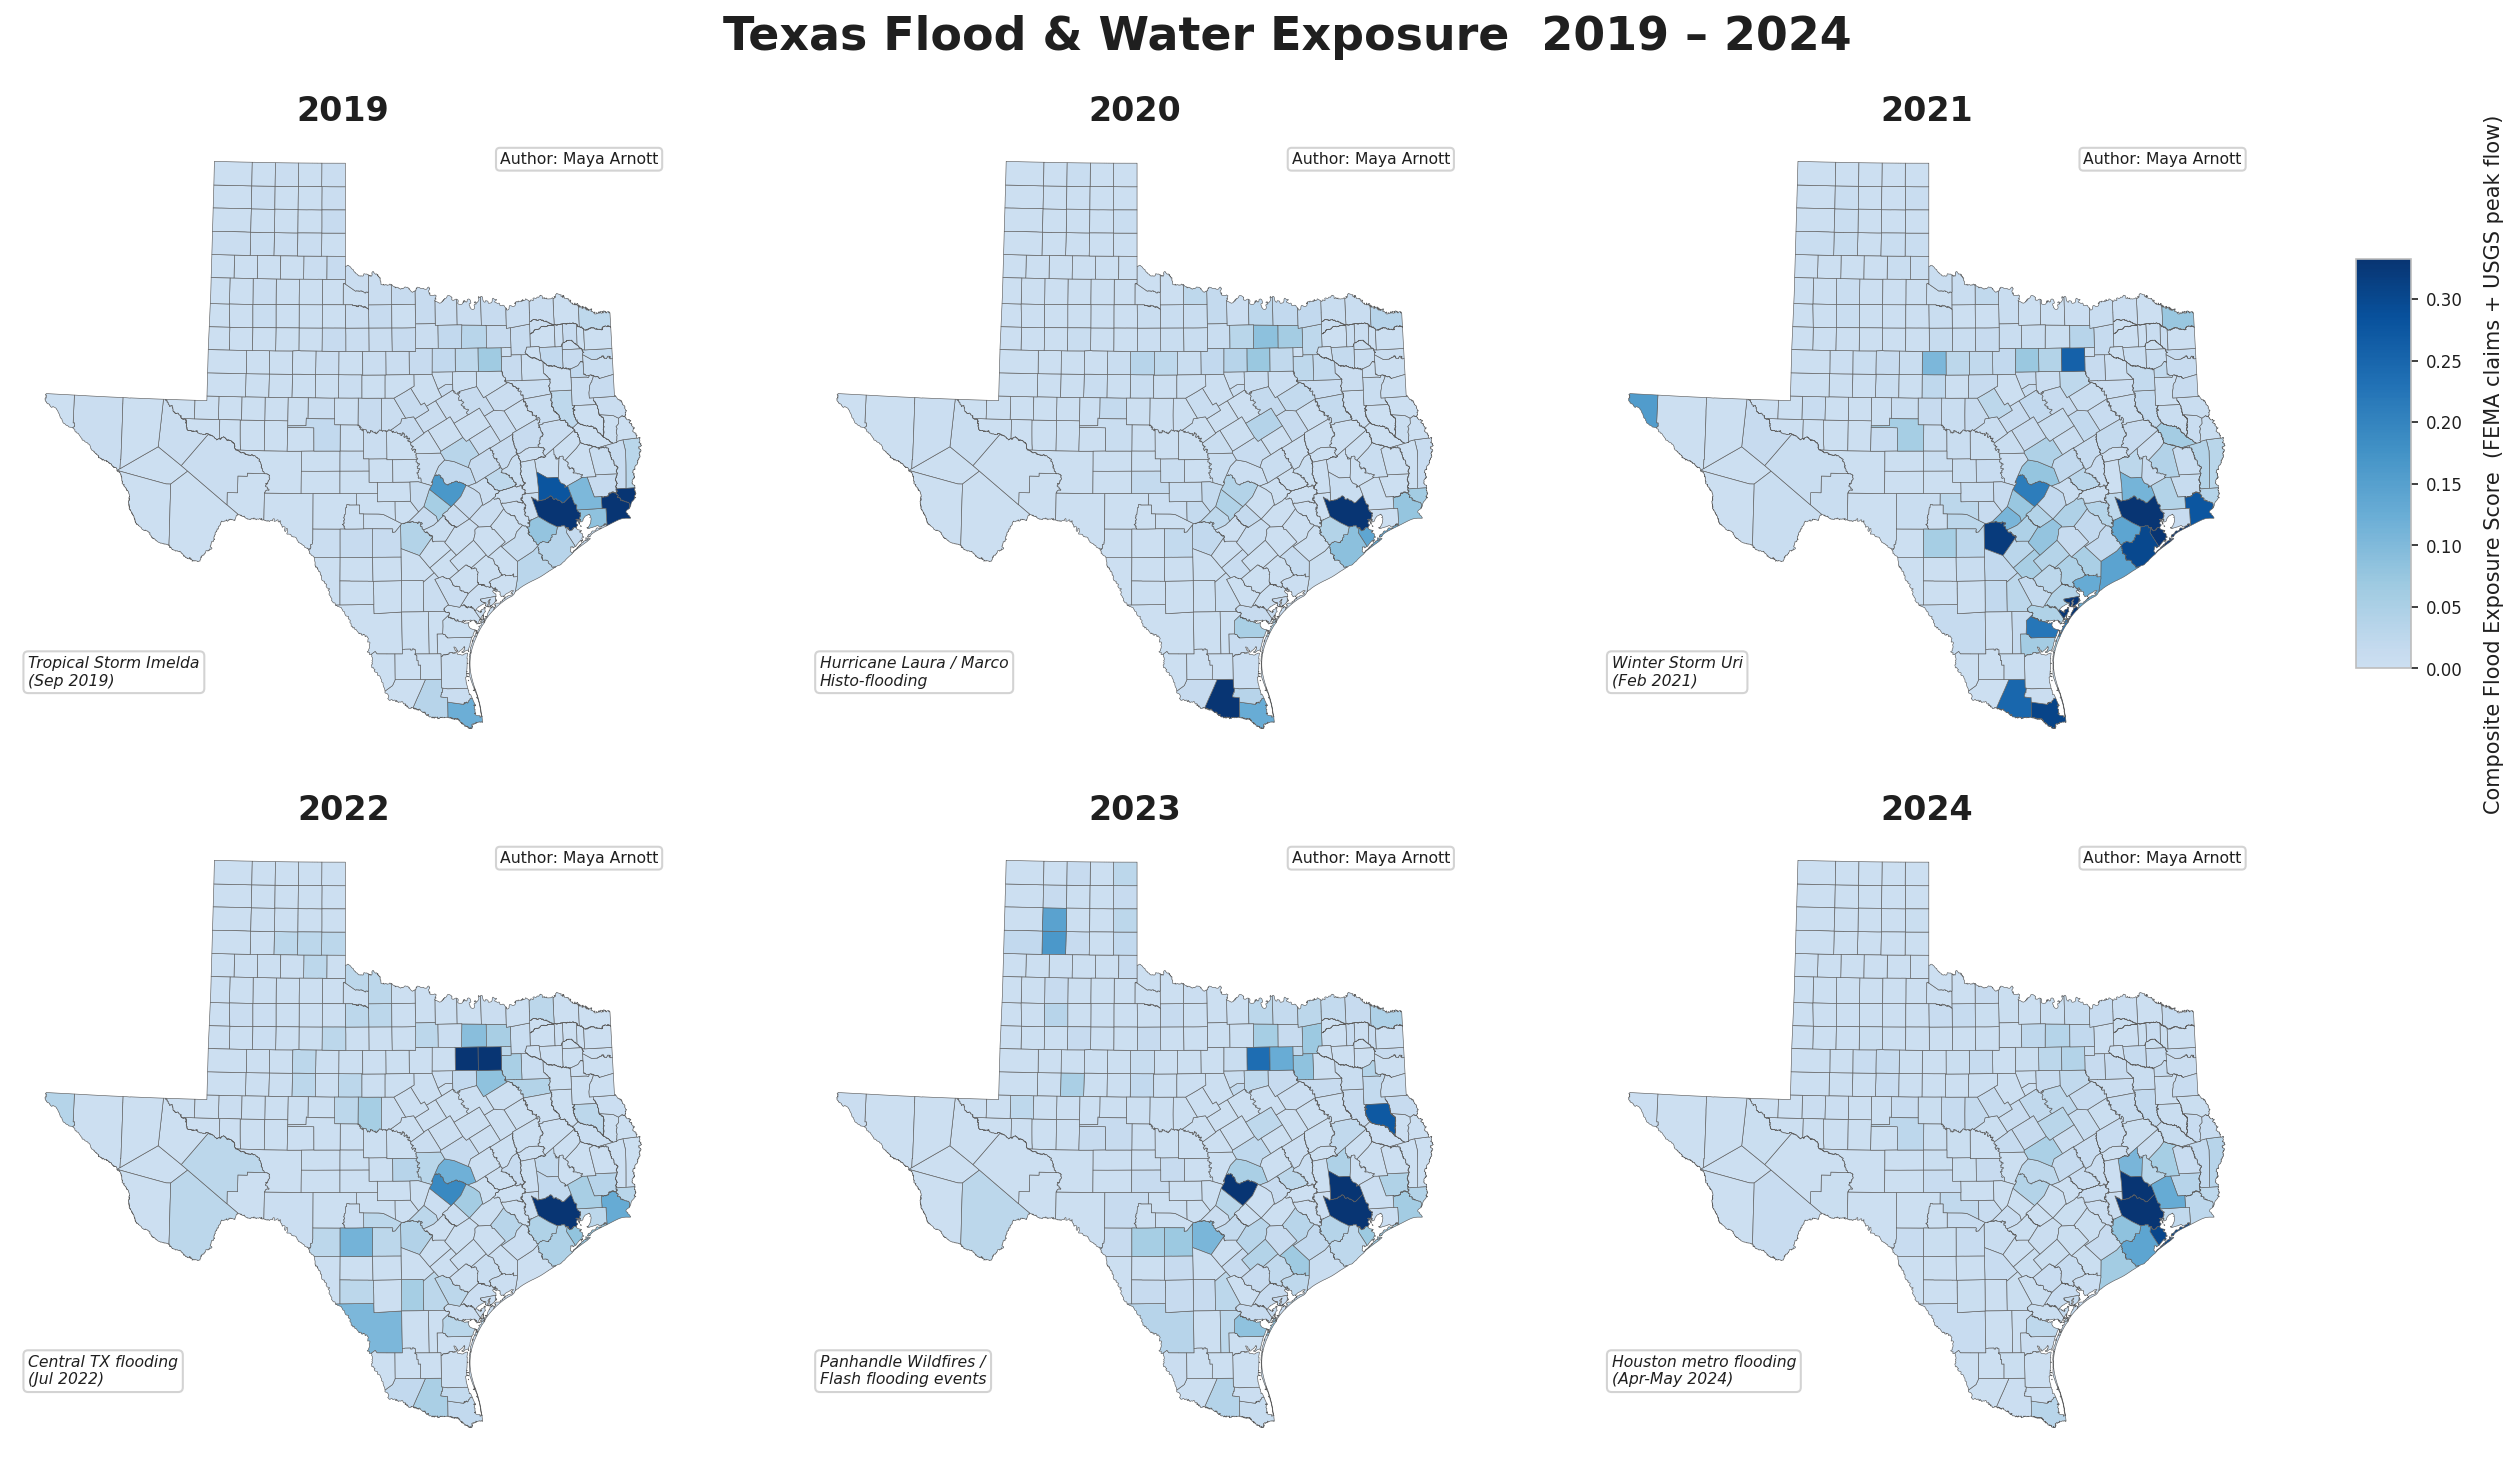
\includegraphics[keepaspectratio]{outputs/texas_flood_grid.png}}

}

\caption{Texas Flood Exposure 2019--2024. Each panel shows the composite
score derived from FEMA NFIP claims and USGS peak streamflow gauge
events. Dashed annotation boxes note the dominant meteorological event
for each year.}

\end{figure}%

Notable patterns:

\begin{itemize}
\tightlist
\item
  \textbf{2019}: Southeast Texas (Harris, Jefferson, Orange counties)
  shows elevated exposure driven by Tropical Storm Imelda, which dropped
  over 40 inches in parts of the region.
\item
  \textbf{2021}: The statewide signal from Winter Storm Uri is visible
  across central and eastern counties, reflecting widespread pipe
  failures and subsequent flood claims rather than riverine flooding
  alone.
\item
  \textbf{2024}: The Houston metropolitan area reemerges as the dominant
  exposure cluster following the April through May flooding events.
\end{itemize}

\subsection{Statewide Trend}\label{statewide-trend}

\begin{figure}[H]

{\centering \pandocbounded{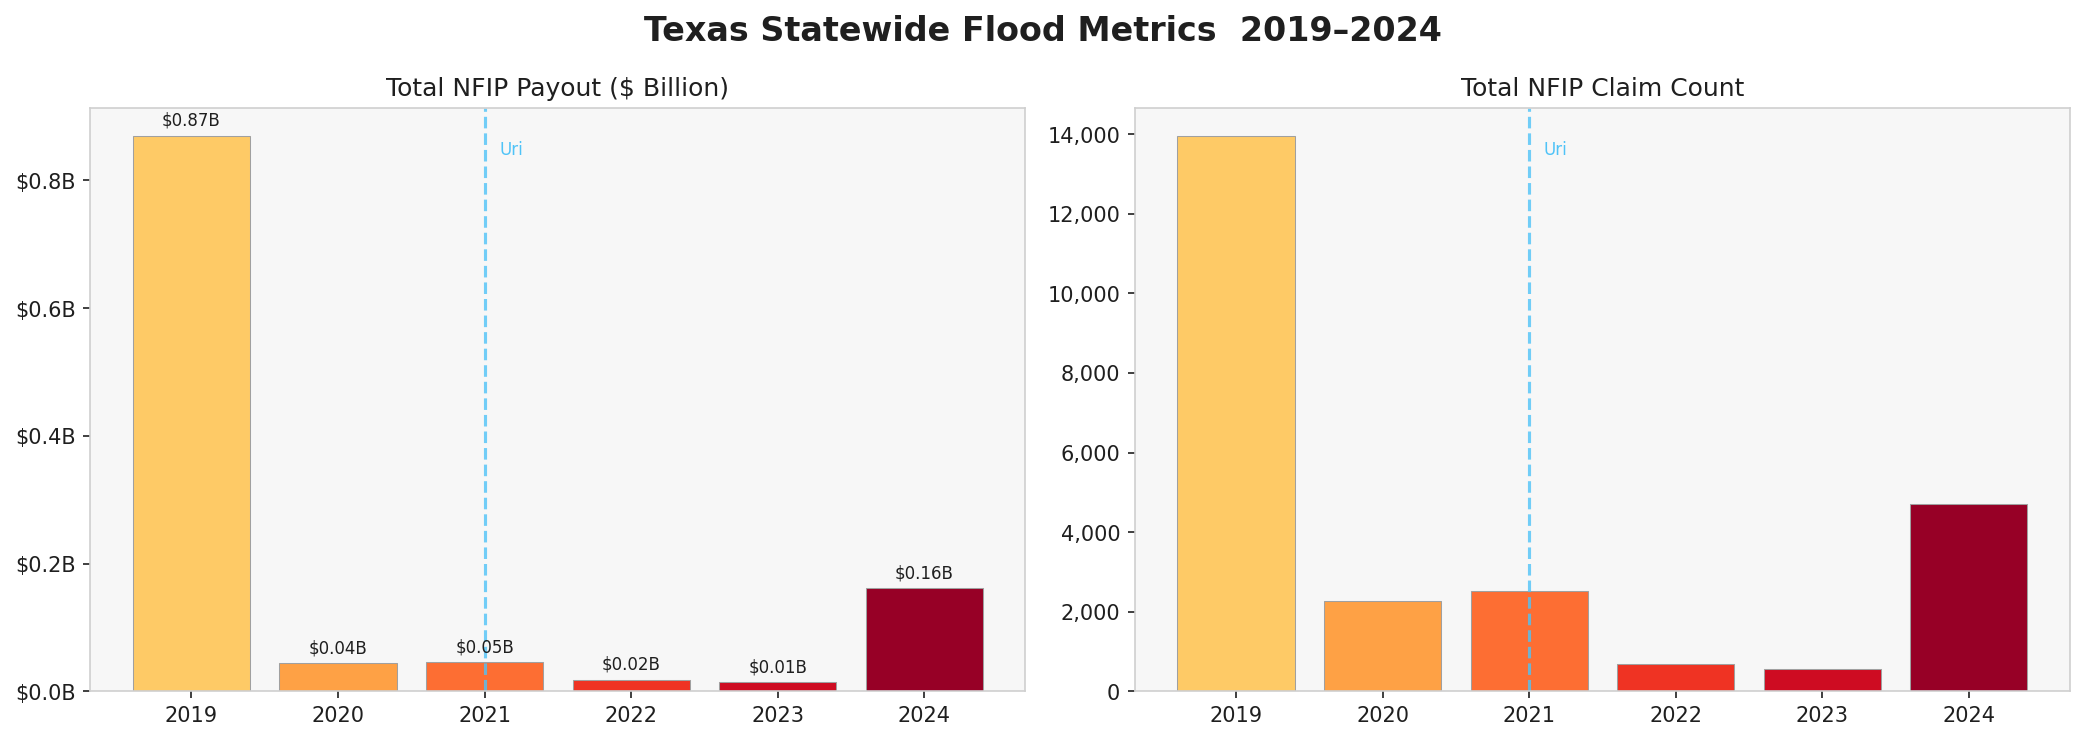
\includegraphics[keepaspectratio]{outputs/texas_flood_statewide.png}}

}

\caption{Total NFIP payout and claim count by year across all Texas
counties. The 2021 Uri spike and the 2024 Houston flooding are
annotated.}

\end{figure}%

\subsection{County Time Series}\label{county-time-series}

The twelve counties with the highest cumulative NFIP payout across
2019--2024 are shown below. Harris County (Houston) dominates by
absolute dollar value, but note that smaller Gulf Coast counties such as
Jefferson and Orange show disproportionately high payouts relative to
their population, indicating structural flood exposure rather than
solely claim volume.

\begin{figure}[H]

{\centering \pandocbounded{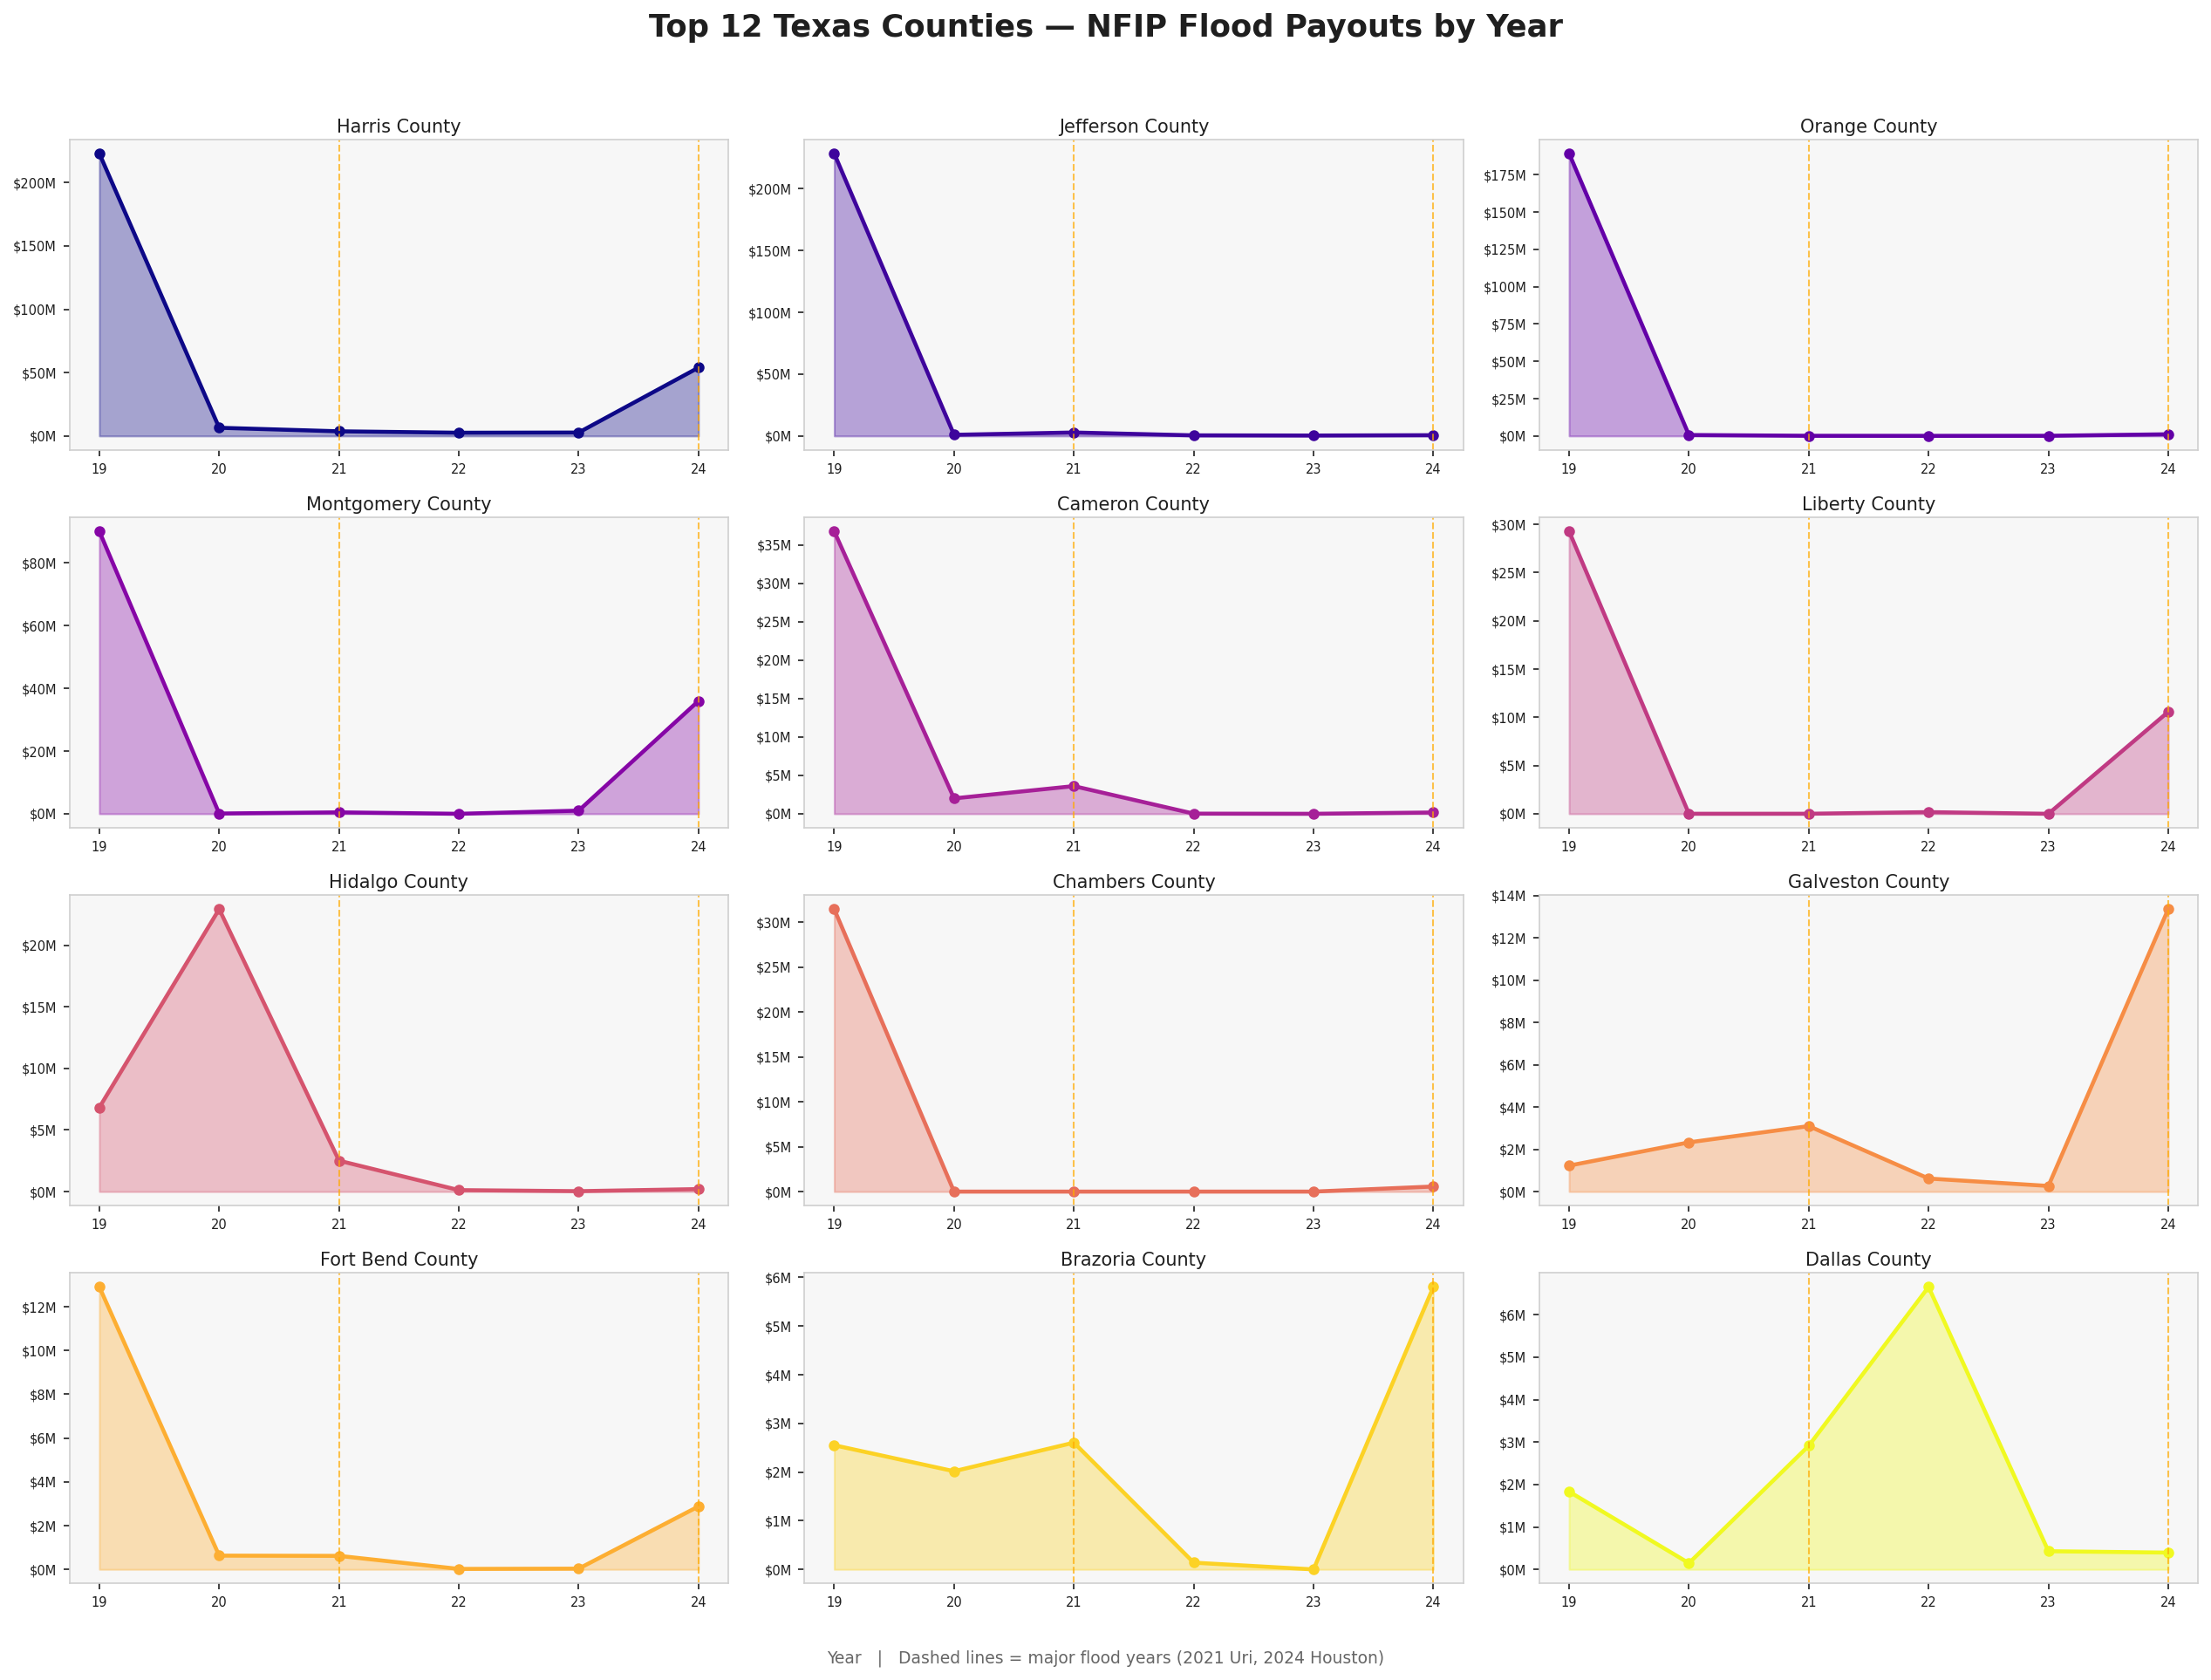
\includegraphics[keepaspectratio]{outputs/texas_flood_timeseries.png}}

}

\caption{NFIP flood payouts by year for the 12 highest-exposure Texas
counties. Dashed vertical lines mark Winter Storm Uri (2021) and the
Houston flooding event (2024).}

\end{figure}%

\begin{center}\rule{0.5\linewidth}{0.5pt}\end{center}

\section{Part 2 --- Flood Frequency
Analysis}\label{part-2-flood-frequency-analysis}

\subsection{Motivation}\label{motivation}

Choropleth maps of historical claims show where damage \emph{has}
occurred. Flood frequency analysis asks a different question: given the
physical hydrology of each county, how large a flood should we expect at
a given return period? This is the core methodology behind FEMA Flood
Insurance Rate Maps and private climate risk scores.

\subsection{Method}\label{method}

The full historical USGS peak streamflow record for Texas --- not just
2019--2024 --- was retrieved to maximize the length of record available
for distribution fitting. Frequency analysis requires ideally 30--50+
years of data to constrain the tail of the distribution.

For each county, annual maximum peak flows were extracted (one value per
year, pooled across all gauges within the county). Two distributions
were fitted:

\textbf{GEV (Generalised Extreme Value)} --- the theoretically justified
model for block maxima such as annual peak flows, derived from extreme
value theory. The GEV has three parameters: location \(\mu\), scale
\(\sigma\), and shape \(\xi\), where the shape parameter determines
whether the tail is bounded (Weibull, \(\xi < 0\)), light (Gumbel,
\(\xi = 0\)), or heavy (Fréchet, \(\xi > 0\)).

\textbf{Log-Pearson III (LP3)} --- the US federal standard for flood
frequency analysis, defined in USGS Bulletin 17C. A Pearson III
distribution is fitted to the log-transformed annual maxima.

Both models were fitted by maximum likelihood. The better fit was
selected by \textbf{AIC} (Akaike Information Criterion):

\[
\text{AIC} = 2k - 2\ln(\hat{L})
\]

where \(k = 3\) parameters and \(\hat{L}\) is the maximized likelihood.
Lower AIC indicates a better fit penalized for model complexity.

From the winning distribution, Q10, Q50, and Q100 return period flows
were estimated --- the flow magnitude with a 1-in-10, 1-in-50, and
1-in-100 annual exceedance probability respectively.

\subsection{Results}\label{results}

\begin{figure}[H]

{\centering \pandocbounded{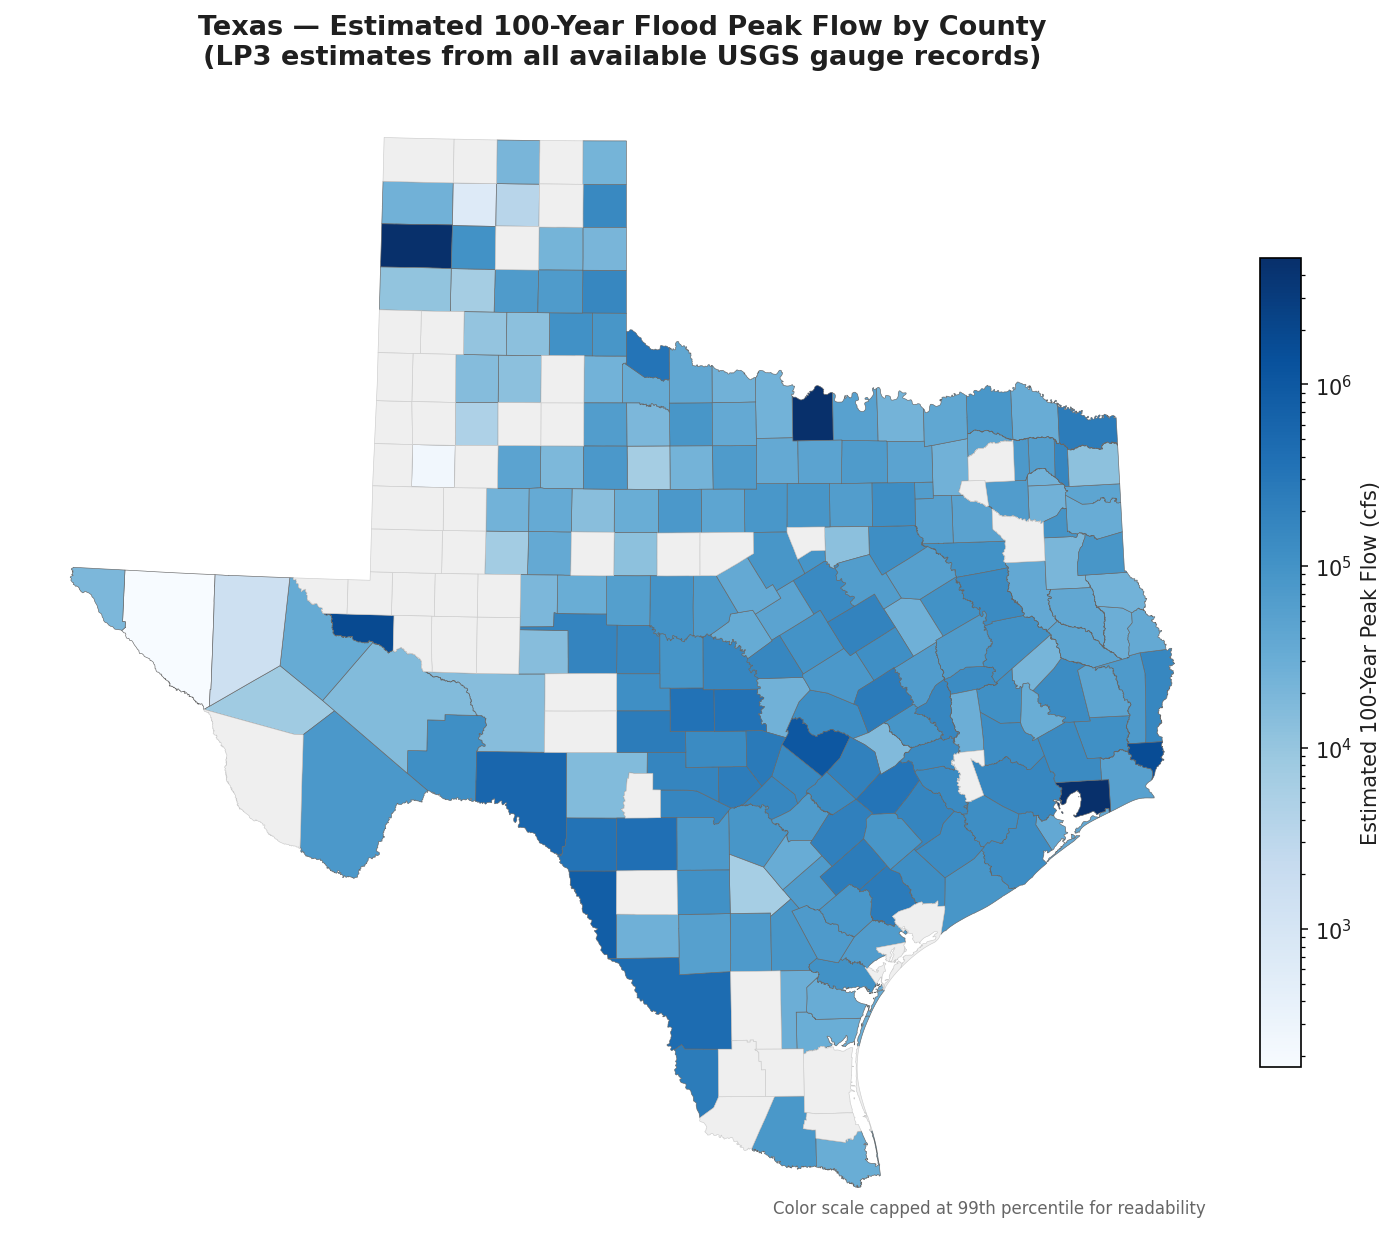
\includegraphics[keepaspectratio]{outputs/texas_return_period_map.png}}

}

\caption{Estimated 100-year peak flow by county. Counties with fewer
than 10 annual observations are shown in grey. The colour scale is
capped at the 99th percentile for readability; East Texas river systems
(Trinity, Neches, Sabine) show the highest estimated 100-year flows.}

\end{figure}%

The frequency curves below show GEV fits for the ten counties with the
most gauge observations. Empirical plotting positions follow the Weibull
formula \(p = m / (n + 1)\) where \(m\) is rank in ascending order.

\begin{figure}[H]

{\centering \pandocbounded{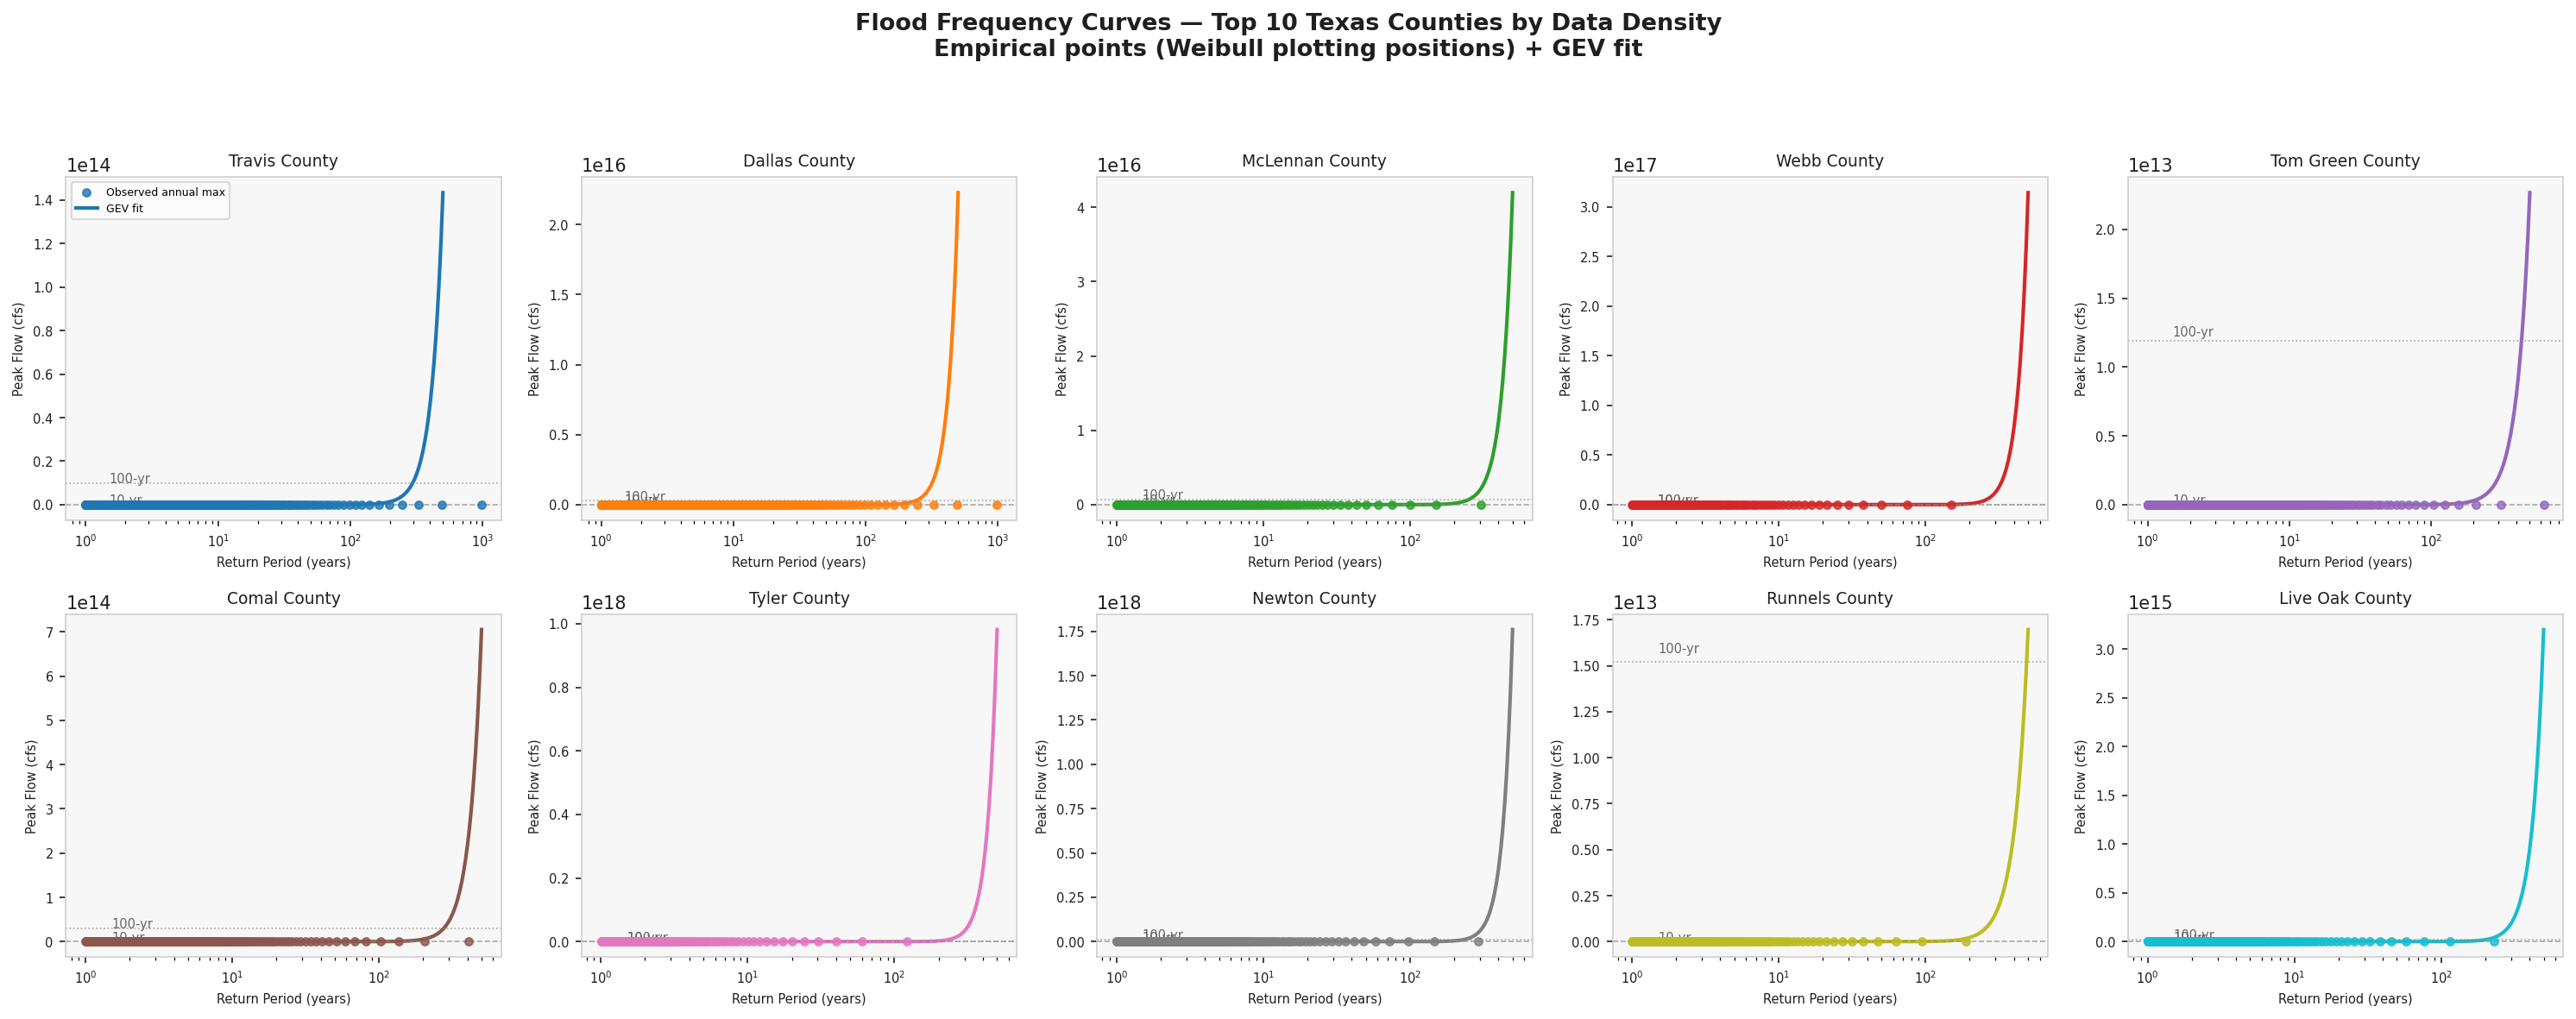
\includegraphics[keepaspectratio]{outputs/texas_flood_frequency_curves.png}}

}

\caption{GEV flood frequency curves for the ten highest-data-density
Texas counties. Points show empirical annual maxima (Weibull plotting
positions); lines show the fitted GEV distribution. Horizontal dashed
lines mark the estimated 10-year and 100-year return flows.}

\end{figure}%

\begin{center}\rule{0.5\linewidth}{0.5pt}\end{center}

\section{Part 3 --- Regression Model}\label{part-3-regression-model}

\subsection{Features}\label{features}

Five predictors were assembled at the county-year level:

{\def\LTcaptype{none} % do not increment counter
\begin{longtable}[]{@{}
  >{\raggedright\arraybackslash}p{(\linewidth - 4\tabcolsep) * \real{0.3333}}
  >{\raggedright\arraybackslash}p{(\linewidth - 4\tabcolsep) * \real{0.3333}}
  >{\raggedright\arraybackslash}p{(\linewidth - 4\tabcolsep) * \real{0.3333}}@{}}
\toprule\noalign{}
\begin{minipage}[b]{\linewidth}\raggedright
Feature
\end{minipage} & \begin{minipage}[b]{\linewidth}\raggedright
Source
\end{minipage} & \begin{minipage}[b]{\linewidth}\raggedright
Rationale
\end{minipage} \\
\midrule\noalign{}
\endhead
\bottomrule\noalign{}
\endlastfoot
\texttt{precip\_anom} & PRISM data converted by Robbie M Parks and
Victoria D Lynch & Annual precipitation deviation from 2019--2024
baseline \\
\texttt{impervious\_pct} & MRLC 2019 & Proportion of county that is
impervious surface; drives runoff \\
\texttt{median\_income} & Census ACS 2022 & Vulnerability proxy; lower
income = fewer mitigation resources \\
\texttt{log\_Q10\_gev} & USGS / GEV fit & Log of 10-year return period
flow; encodes baseline flood hazard \\
\texttt{year\_trend} & Derived & Linear year index; captures any secular
trend in claims \\
\end{longtable}
}

The target variable is \(\log(1 + \text{claim count})\) --- the log
transform stabilizes the right-skewed distribution of claim counts,
where most county-years have zero or few claims but a small number have
thousands.

\subsection{OLS}\label{ols}

An OLS model with heteroscedasticity-robust standard errors (HC3) was
fitted to the full 2019--2024 panel. HC3 standard errors are preferred
here because variance in claim counts is substantially higher in
flood-prone counties than in dry ones --- a classic case of
heteroscedasticity.

\[
\log(1 + y_{it}) = \beta_0 + \beta_1 \cdot \text{precip\_anom}_t +
\beta_2 \cdot \text{imperv}_i + \beta_3 \cdot \text{income}_i +
\beta_4 \cdot \log Q10_i + \beta_5 \cdot \text{trend}_t + \varepsilon_{it}
\]

\textbf{In-sample R² = 0.464.} The five features explain about 46.4\% of
variance in log claim counts.

\subsection{Random Forest}\label{random-forest}

The same features were passed to a Random Forest with 300 trees, maximum
depth 6, and minimum 5 samples per leaf. \textbf{5-fold cross-validated
R² = 0.361 ± 0.083, and the temporal holdout (2023--2024) R² = 0.603.}

The higher in-sample R² (≈0.748) reflects the model's fit to the
training data and illustrates that Random Forest can flexibly capture
non-linear and interaction effects that OLS cannot. The improvement over
OLS indicates two things: 1. Relationships between features and claim
counts are non-linear. For example, impervious surface likely has little
effect until it crosses a threshold, beyond which runoff and claims
increase sharply. 2. Interaction effects matter: a county that is both
highly paved and experiences an anomalously wet year sees
disproportionately more claims than either factor alone would predict.

These patterns are captured naturally by Random Forest without manual
feature engineering, but the low 5-fold cross-validation R² suggests
that the model may be overfitting to specific years in the training
data, particularly given the small sample size (762 county-year rows).
The temporal holdout validation below provides a more realistic test of
generalization to new years.

\begin{figure}[H]

{\centering \pandocbounded{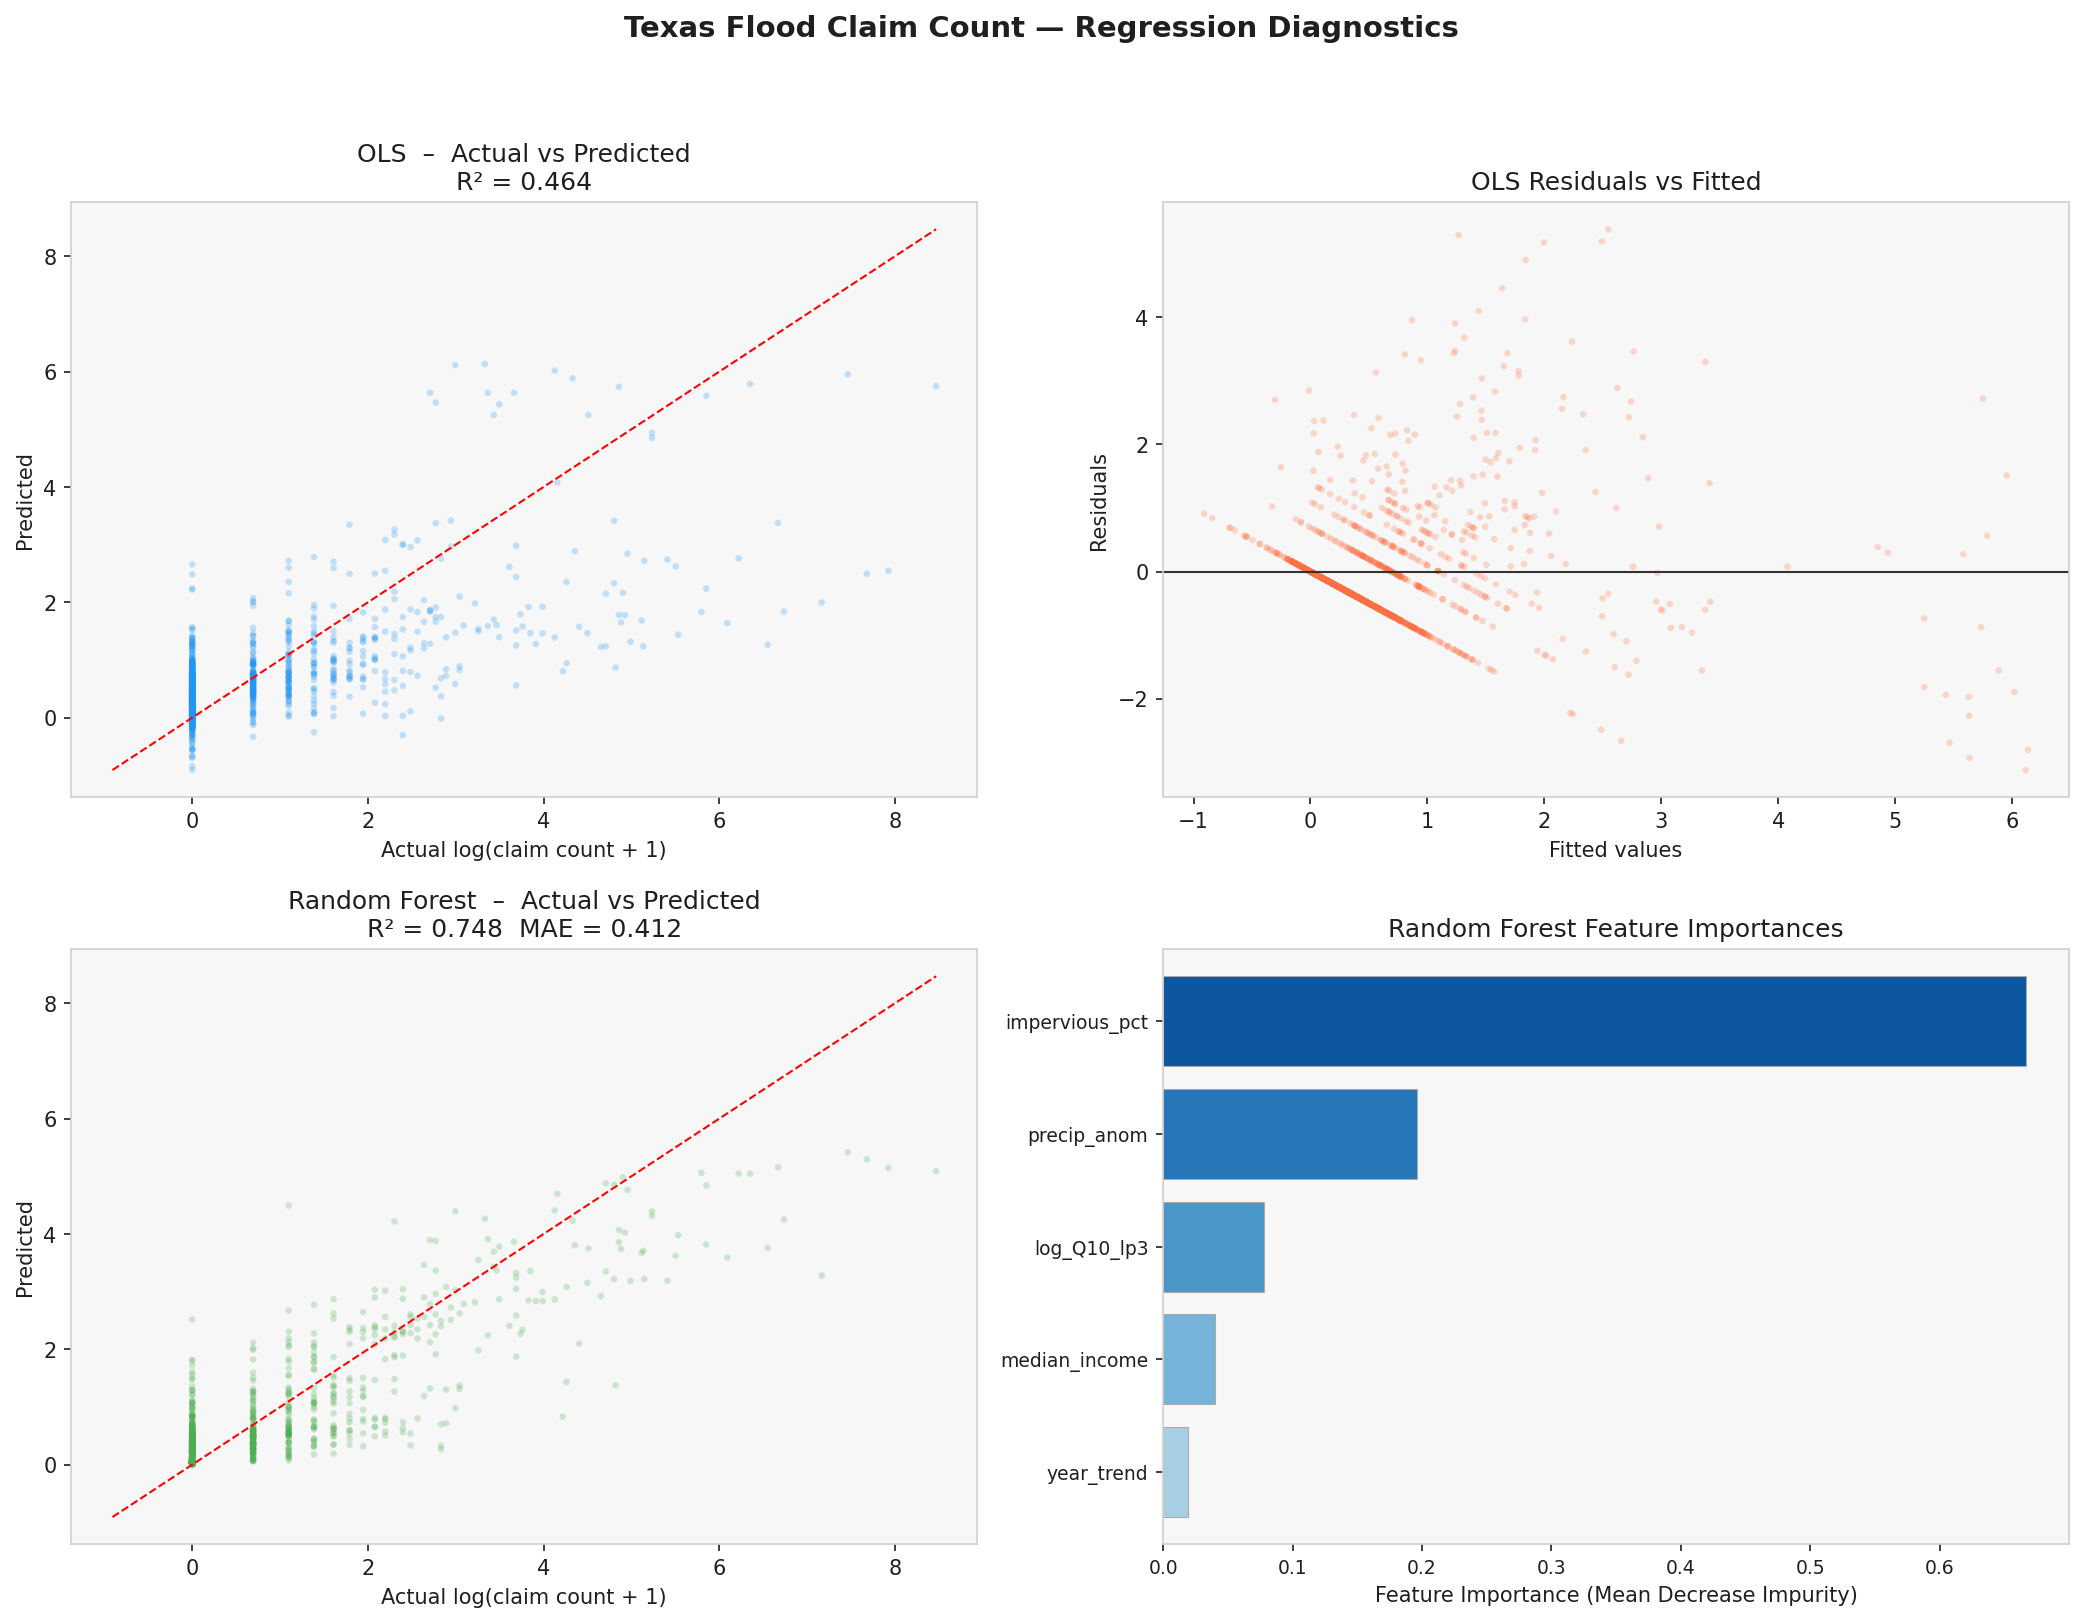
\includegraphics[keepaspectratio]{outputs/texas_regression_actual_vs_pred.png}}

}

\caption{Regression diagnostics. Top row: OLS actual vs predicted and
residual plot. Bottom row: Random Forest actual vs predicted and feature
importances. The fan shape in the OLS residual plot confirms
heteroscedasticity --- variance increases with fitted values, consistent
with a skewed claim distribution.}

\end{figure}%

\begin{center}\rule{0.5\linewidth}{0.5pt}\end{center}

\section{Part 4 --- Temporal Holdout
Validation}\label{part-4-temporal-holdout-validation}

\subsection{Why Temporal Holdout
Matters}\label{why-temporal-holdout-matters}

The 5-fold cross-validation above splits data randomly. This means a
fold can train on 2022 and 2023 data and then predict 2020 --- leaking
future information into training. For a forecasting application, this is
too optimistic: in practice a model trained on historical data will only
ever be applied to future years it has never seen.

A temporal holdout enforces the correct discipline: train exclusively on
2019--2022, then evaluate on 2023--2024 as if making genuine
out-of-sample predictions.

\begin{verbatim}
Training:  2019–2022  (~1,016 county-year rows)
Test:      2023–2024  (~508 county-year rows)
\end{verbatim}

\subsection{Results}\label{results-1}

{\def\LTcaptype{none} % do not increment counter
\begin{longtable}[]{@{}llll@{}}
\toprule\noalign{}
Model & CV R² & Holdout R² & Change \\
\midrule\noalign{}
\endhead
\bottomrule\noalign{}
\endlastfoot
OLS & 0.464 & 0.443 & −0.112 \\
Random Forest & 0.361 & 0.603 & +0.242 \\
\end{longtable}
}

\begin{figure}[H]

{\centering \pandocbounded{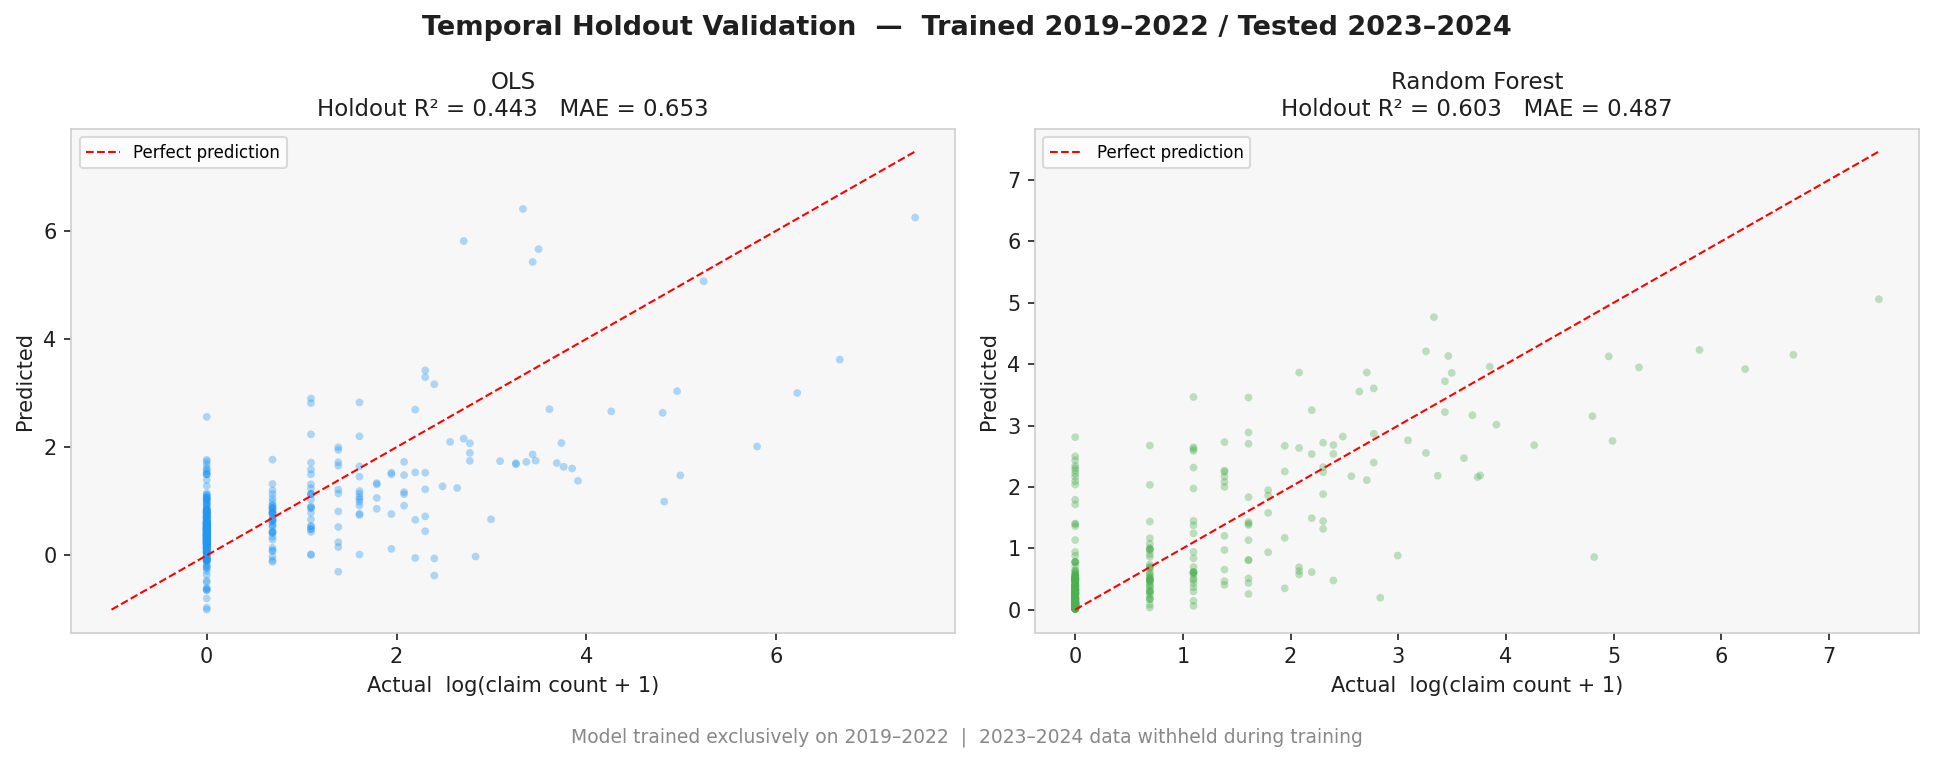
\includegraphics[keepaspectratio]{outputs/texas_temporal_holdout.png}}

}

\caption{Temporal holdout validation. Both models trained on 2019--2022
only and evaluated on withheld 2023--2024 data.}

\end{figure}%

\subsection{Interpretation}\label{interpretation}

The OLS holdout R² of 0.443 indicates that the linear relationships
learned from 2019--2022 generalize reasonably well to new years. While
some degradation is expected, the linear model still retains much of its
explanatory power.

The Random Forest achieved a holdout R² of 0.603, which is an
improvement over its 5-fold CV R² of 0.361. This suggests that the
non-linear patterns it captured, particularly the interaction between
impervious surface and flood hazard, are genuine and temporally stable
rather than artifacts of overfitting to specific training years.

\section{The remaining unexplained variance is likely due to the absence
of event-level inputs. Incorporating NOAA storm footprints or FEMA
disaster declaration indicators as county-year features would provide
the spatial and temporal specificity that the current statewide
precipitation anomaly lacks, and would likely be the single best
addition for boosting holdout R²
further.}\label{the-remaining-unexplained-variance-is-likely-due-to-the-absence-of-event-level-inputs.-incorporating-noaa-storm-footprints-or-fema-disaster-declaration-indicators-as-county-year-features-would-provide-the-spatial-and-temporal-specificity-that-the-current-statewide-precipitation-anomaly-lacks-and-would-likely-be-the-single-best-addition-for-boosting-holdout-ruxb2-further.}

\section{Part 5 --- Final Risk Index}\label{part-5-final-risk-index}

A county-level risk index was constructed by combining four normalized
dimensions:

\[
\text{Risk Index} = 0.40 \cdot \text{Exposure} + 0.35 \cdot \text{Hazard} +
0.15 \cdot \text{Imperviousness} + 0.10 \cdot \text{Vulnerability}
\]

where:

\begin{itemize}
\tightlist
\item
  \textbf{Exposure} = total NFIP claims across 2019--2024, normalized
  0--100
\item
  \textbf{Hazard} = estimated Q100 return period flow, normalized 0--100
\item
  \textbf{Imperviousness} = mean impervious surface \%, normalized
  0--100
\item
  \textbf{Vulnerability} = inverse of median household income,
  normalized 0--100 (lower income = higher vulnerability)
\end{itemize}

The full table is saved to
\texttt{outputs/texas\_risk\_score\_final.csv}.

\begin{center}\rule{0.5\linewidth}{0.5pt}\end{center}

\section{Limitations \& Next Steps}\label{limitations-next-steps}

\textbf{Current limitations:}

\begin{verbatim}
•   Precipitation data is now county-specific rather than statewide, which has improved the OLS model’s ability to predict log claim counts. However, it still only captures annual totals. Short-term, event-level rainfall variability within the year is still lost.
•   Impervious surface and income are static and do not capture year-on-year changes in land use or economic conditions.
•   No event-level storm footprints or FEMA disaster indicators are included. Flood damage is fundamentally event-driven and spatially concentrated, so aggregating to the county-year level still loses much of that resolution. These remain the main factors limiting holdout performance, particularly for the Random Forest model.
\end{verbatim}

\textbf{Next Steps:}

\begin{enumerate}
\def\labelenumi{\arabic{enumi}.}
\tightlist
\item
  Add a binary FEMA disaster declaration indicator per county-year as a
  feature, which is publicly available and would directly encode whether
  a major event occurred
\item
  Implement a proper train/test split by event rather than by year,
  treating each named storm as a holdout event
\item
  Incorporate NLCD impervious surface rasters over the years directly to
  enable time-varying land cover from the 2001, 2006, 2011, 2016, and
  2021 NLCD vintages
\end{enumerate}

\begin{center}\rule{0.5\linewidth}{0.5pt}\end{center}

\section{Reproducibility}\label{reproducibility}

\begin{Shaded}
\begin{Highlighting}[]
\CommentTok{\# Run in order}
\ExtensionTok{python}\NormalTok{ texas\_flood\_analysis.py}
\ExtensionTok{python}\NormalTok{ risk\_modeling.py}
\end{Highlighting}
\end{Shaded}

All outputs are written to \texttt{./outputs/}. The Quarto document can
be rendered with:

\begin{Shaded}
\begin{Highlighting}[]
\ExtensionTok{quarto}\NormalTok{ render texas\_flood\_analysis.qmd}
\end{Highlighting}
\end{Shaded}





\end{document}
